\section{Ideal potential flows (continued) (37-44)}

\begin{framed}
\textbf{Opening remark:} 2-dimensional potential flow solutions will often look like
\begin{equation}
\Phi(x,y) = u_\infty x + f(x,y).
\end{equation}
Any function $f(x,y)$, which fulfills
\begin{equation}
\ppdiff{f}{x}+\ppdiff{f}{y}=0 \qquad \mathrm{and}\qquad f(|x|,|y|\rightarrow\infty) = 0,
\end{equation}
describes a flow around some obstacle.
\end{framed}


\textbf{Play 1:}
\begin{equation}
\Phi(x,y)=\frac{m}{2\pi} \ln \sqrt{x^2+y^2}
\end{equation}
represents the radial flow resulting from a source with strength $m$. See \fref{fig:radial-streamlines}.
\begin{figure}[!h]
    \centering
    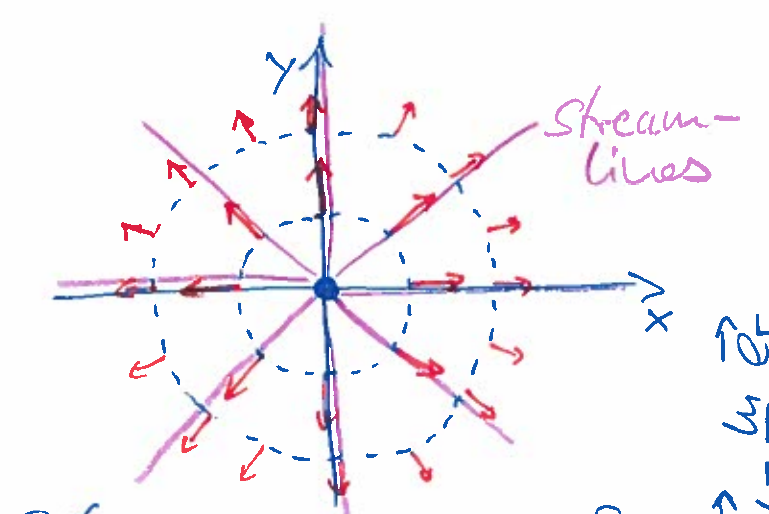
\includegraphics[width=.5\textwidth]{week3/radial-streamlines}\\
    \caption{}
    \label{fig:radial-streamlines}
\end{figure}

\textbf{Play 2:} method of images. Source flow in front of a wall. See \fref{fig:mirror-source}.

Boundary condition: no flow through the wall; only tangential component.
\begin{equation}
\phi(x,y) = \frac{m}{2\pi}\ln\sqrt{(x+a)^2+y^2} + \frac{m}{2\pi}\ln\sqrt{(x-a)^2+y^2}
\end{equation}
\begin{figure}[!h]
    \centering
    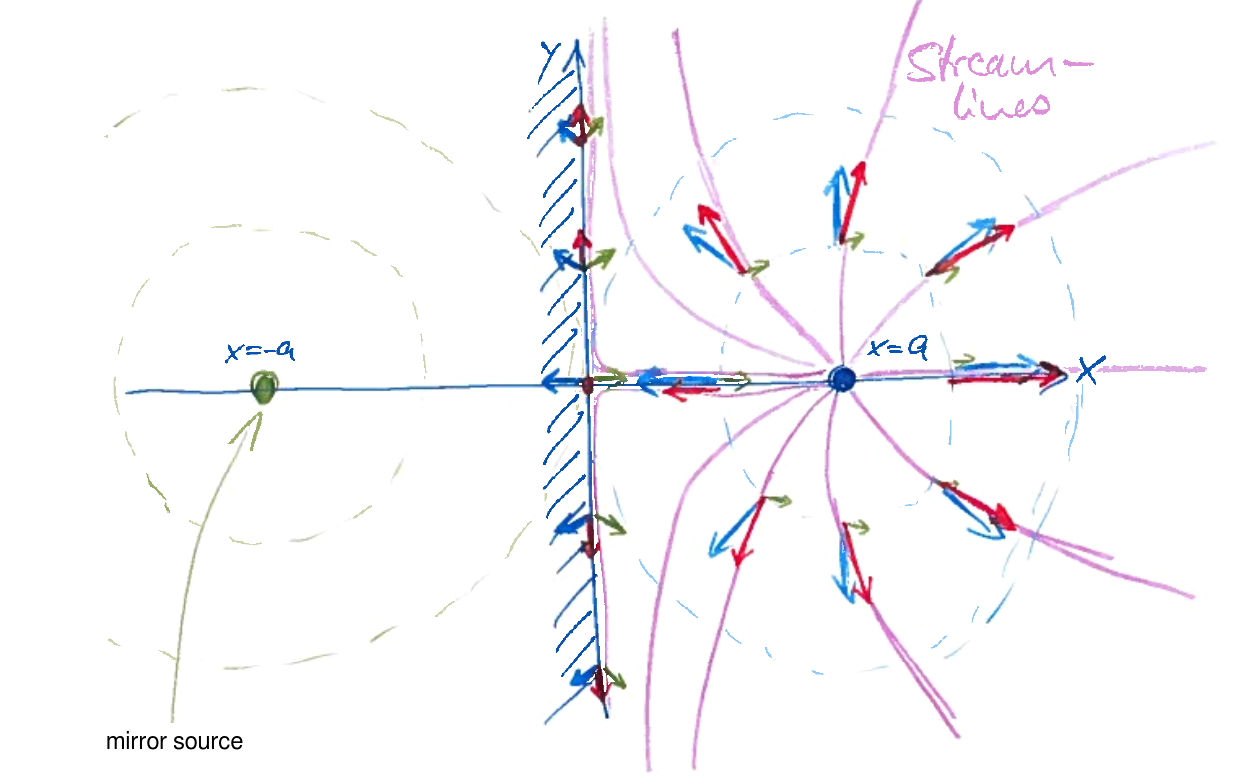
\includegraphics[width=.6\textwidth]{week3/mirror-source}\\
    \caption{}
    \label{fig:mirror-source}
\end{figure}

\textbf{Play 3:} flow past a 2-dimensional half-body. See \fref{fig:half-body}.
\begin{align}
\Phi &= u_\infty x + \frac{m}{2\pi}\ln\sqrt{x^2+y^2}\\
\leadsto
\ppdiff{\Phi}{x}+\ppdiff{\Phi}{y} &= 0
\end{align}
\begin{align}
u_x(x,y) &= u_\infty + \frac{m}{2\pi}\frac{x}{x^2+y^2}\\
u_y(x,y) &= u_\infty + \frac{m}{2\pi}\frac{y}{x^2+y^2}
\end{align}

Engineering flow interpretations:
\begin{enumerate}
\item An example of the beginning of the half-body is the leading edge of an airfoil
\item pedestrian on a bridge looking down: front part of a bridge pier
\item flow over a cliff
\end{enumerate}

\begin{figure}[!h]
    \centering
    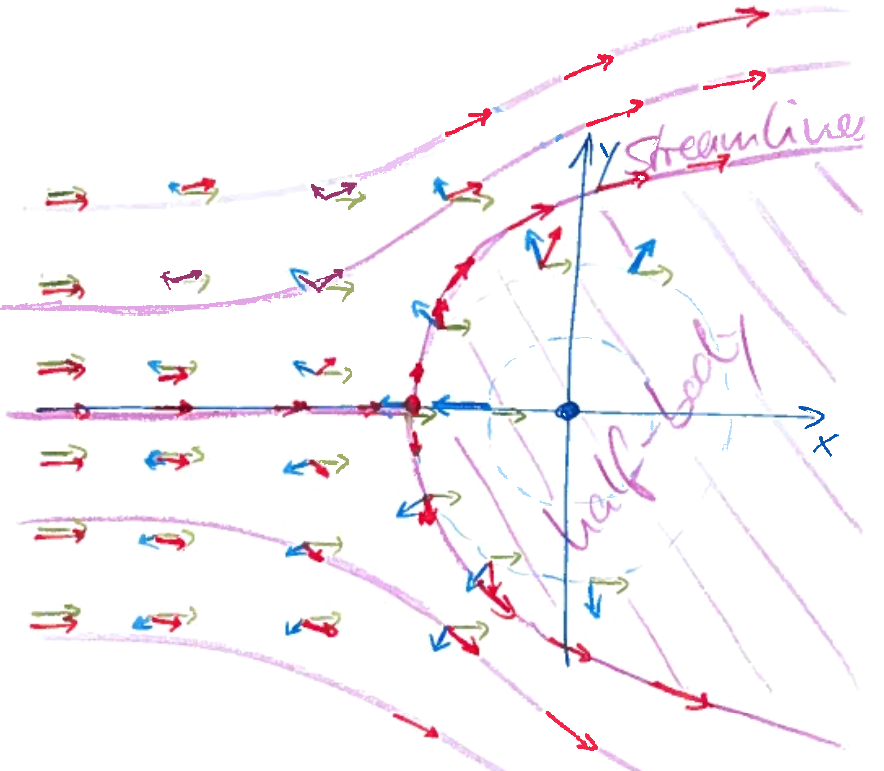
\includegraphics[width=.6\textwidth]{week3/half-body}\\
    \caption{}
    \label{fig:half-body}
\end{figure}

\textbf{Play 4:} numerial solutions (KCD section 6: Computational Fluid Dynamics)

\textbf{Play 5:} "beauty of mathematics". Conformal mappings.
Complex potential
\begin{equation}
w(z) = \phi(x,y)+i\psi(x,y)
\end{equation}
where $z=x+iy$.

Velocity:
\begin{align}
\diff{w(z)}{z} &= \diff{w(z)}{z}\biggm\vert_{dz=dx} = \pdiff{\phi}{x}+i\pdiff{\psi}{x} = u_x-iu_y \\
&= \diff{w(z)}{z}\biggm\vert_{dz=idy} = \pdiff{\phi}{y}+i\pdiff{\psi}{y} = \pdiff{\psi}{y}-i\pdiff{\phi}{y} = u_x-iu_y
\end{align}

Differentiable example 1:
\begin{equation}
w(z)=u_\infty z = u_\infty(x+iy) = u_\infty x + iu_\infty y
\end{equation}
describes the constant flow $\vec{u}=u_\infty \vec{e}_x$.

Differentiable example 2:
\begin{align}
w(z) &= \frac{m}{2\pi}\ln z = \frac{m}{2\pi} \ln(x+iy)\\
&= \frac{m}{2\pi}\ln(re^{i\theta}\\
&= \frac{m}{2\pi}\ln r +\frac{m}{2\pi}\ln e^{i\theta}\\
&= \frac{m}{2\pi}\ln\sqrt{x^2+y^2} + i\frac{m}{2\pi}\theta
\end{align}
The two terms in the last line is the velocity field and stream function of a radial source flow (see "play 1").

Differentiable example 3:
\begin{align}
w(z) &= \frac{A}{2}z^2 = \frac{A}{2}(x+iy)^2\\
&= \frac{A}{2}(x^2-y^2)+iAxy
\end{align}

Differentiable example 4:
\begin{align}
w(z) &= \phi(x,y) +i\psi(x,y) = u_\infty x\left(1+\frac{R^2}{x^2+y^2}\right) + iu_\infty y \left(1-\frac{R^2}{x^2+y^2}\right) \\
& =u_\infty(x+iy) + u_\infty R^2\frac{x-iy}{x^2+y^2} \\
&= u_\infty(x+iy)+\frac{u_\infty R^2}{x+iy}\\
&= u_\infty\left(z+\frac{R^2}{z}\right)
\end{align}

flow around cylinder with radius $R$:
\begin{equation}
w(z)=u_\infty\left(z+\frac{R^2}{z}\right)
\end{equation}
change of variable:
\begin{equation}
z)z(\tilde{z})
\end{equation}
Example:
\begin{align}
\tilde{z} &= (z+z_0)+\frac{1}{z+z_0}\\
\leadsto
w_\mathrm{new\ obstacle}(\tilde{z}) &= w_\mathrm{cylinder}(z(\tilde{z}))
\end{align}

\begin{shaded}
Should we include the figure on the left half of page 43 here?
\end{shaded}


\begin{framed}
\textbf{Remark:} other applications of conformal mappings

\textbf{Electrostatics}
\begin{equation}
\Delta\phi = \vec{\nabla}\cdot\vec{\nabla\phi=0}
\end{equation}

\textbf{Heat flux}
\begin{equation}
\pdiff{T(x,y)}{t}=\kappa\vec{\nabla}\cdot\vec{\nabla}T(x,y) \Rightarrow \Delta T(x,y) = 0
\end{equation}
\end{framed}
